\chapter{Potencial eléctrico }
Cuando una partícula con carga se mueve en un campo eléctrico, el campo ejerce una fuerza que efectúa \textit{trabajo} sobre la partícula. Este trabajo siempre se puede expresar en términos de la energía potencial eléctrica\footnote{O simplemente \textit{potencial eléctrico} o \textit{potencial}}. Una diferencia de potencial entre un punto y otro reciba el nombre de \textit{voltaje}.

\section{Energía potencial eléctrica}
Cuando una fuerza $\vec{F}$ actúa sobre una partícula que se mueve de un punto $a$ a un punto $b$, el trabajo $W_{a\to b}$ efectuado por la fuerza está dado por la siguiente \textit{integral de línea}:

\begin{equation}\label{23.1}\marginnote{Trabajo realizado por una fuerza}
W_{a\to b}=\int_a^b\vec{F}\cdot d\vec{l}=\int_a^bF\cos\phi dl
\end{equation}

donde $d\vec{l}$ es un desplazamiento infinitisimal a lo largo de la trayectoria de la partícula, y $\phi$ es el ángulo entre $\vec{F}$ y $d\vec{l}$ 	en cada punto de la trayectoria.

Si la fuerza $\vec{F}$ es \textit{conservativa}, el trabajo realizado por esta siempre se puedo expresar en términos de una \textbf{energía potencial} $U$. Cuando la partícula se mueve de un punto donde la energía potencial es $U_a$ a otro donde es $U_b$, el cambio de energía potencial es $\Delta U=U_b-U_a$, y el trabajo $W_{a\to b}$ que realiza la fuerza es

\begin{equation}\label{23.2}\marginnote{Trabajo efectuado por una fuerza conservativa}
\boxed{W_{a\to b}=U_a-U_b=-(U_b-U_a)=-\Delta U}
\end{equation}

En tercer lugar, el teorema del trabajo y la energía establece que el cambio en la energía cinética $\Delta K=K_b+K_a$ durante cualquier desplazamiento es igual al trabajo \textit{total} realizado sobre la partícula. Si el único trabajo efectuado sobre la partícula lo realizan fuerzas conservativas, entonces la ecuación \ref{23.2} da el trabajo total, y $K_b-K_a=-(U_b-U_a)$. Es decir, 

\begin{equation}\label{23.3}
K_a+U_a=K_b+U_b
\end{equation}

Es decir, en estas circunstancias, la energía mecánica total (cinética más potencial) se
\textit{conserva}.

\subsection{Energía potencial eléctrica de un campo uniforme}
\begin{figure}[h]
\centering
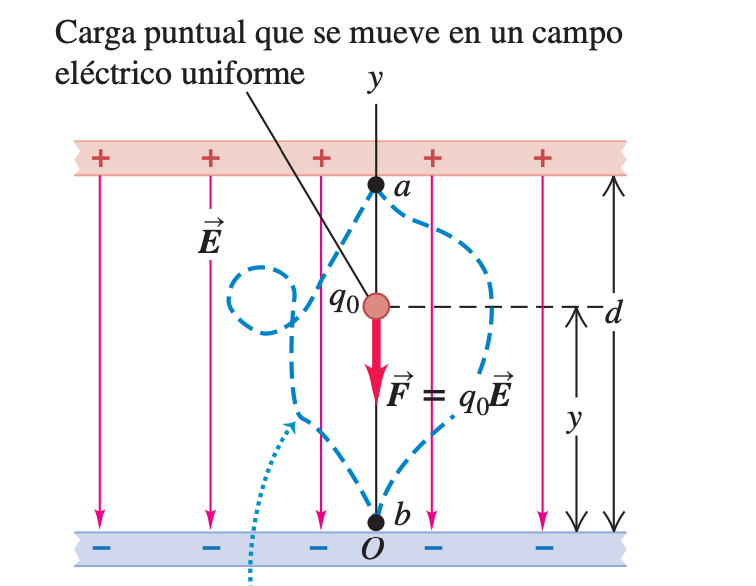
\includegraphics[scale=0.5]{fig/energia_potencial}
\caption{Trabajo realizado sobre una carga puntual que se mueve en un campo eléctrico uniforme. El trabajo realizado por la fuerza eléctrica es el mismo para cualquier trayectoria de $a$ a $b$: $W_{a\to b}=-\Delta U=q_0Ed$} 
\label{fig:energia_potencial}
\end{figure}

En la figura \ref{fig:energia_potencial} un par de placas metálicas paralelas con carga generan un campo eléctrico uniforme descendente y con magnitud $E$. El campo ejerce una fuerza hacia abajo con magnitud $F=q_0E$ sobre una carga de prueba positiva $q_0$. A medida que la carga se mueve hacia abajo una distancia $d$ del punto $a$ al punto $b$, la fuerza sobre la carga de prueba es constante e independiente de su localización. Por lo tanto, el trabajo realizado por el campo eléctrico es 

\begin{equation}\label{23.4}
W_{a\to b}=Fd=q_0Ed
\end{equation}

Este trabajo es positivo, toda vez que la fuerza está en la misma dirección que el desplazamiento neto de la carga de prueba. Este trabajo puede representarse con una función de \textbf{energía potencial} $U$, que para la fuerza eléctrica está dada por

\begin{equation}\label{23.5}
U=q_0Ey
\end{equation}

Cuando la carga de prueba se mueve de la altura $y_a$ a la altura $y_b$, el trabajo realizado sobre la carga por el campo está dado por

\begin{equation}\label{23.6}
W_{a\to b}=-\Delta U=-(U_b-U_a)=-(q_0Ey_b-q_0Ey_a)=q_0E(y_a-y_b)
\end{equation}

\subsection{Energía potencial entre dos cargas puntuales}
El concepto de energía potencial se puede aplicar a una carga puntual en \textit{cualquier} campo eléctrico generado por una distribución de carga estática. 
Cualquier distribución de carga se representa como un conjunto de cargas puntuales. Por consiguiente, es útil calcular el trabajo realizado sobre una carga de prueba $q_0$ que se mueve en el campo eléctrico ocasionado por una sola carga puntual estacionaria $q$.

En primer lugar se considerará un desplazamiento a lo largo de una línea radial, del punto $a$ al punto $b$. La fuerza sobre $q_0$ está dada por la ley de Coulomb, y su componente radial es

\begin{equation}\label{23.7}
F_r=\frac{1}{4\pi\epsilon_0}\frac{qq_0}{r^2}
\end{equation}

Si $q$ y $q_0$ tienen el mismo signo, la fuerza es de repulsión y $F_r$ es positiva; en caso contrario la fuerza es de atracción y $F_r$ es negativa. La fuerza \textit{no} es constante durante el desplazamiento, y se tiene que integrar para obtener el trabajo $W_{a\to b}$ que realiza esta fuerza sobre $q_0$a medida que $q_0$ se mueve de $a$ a $b$

\begin{equation}\label{23.8}
W_{a\to b}=\int_{r_a}^{r_b}F_rdr=\int_{r_a}^{r_b}\frac{1}{4\pi\epsilon_0}\frac{qq_0}{r^2}dr=\frac{qq_0}{4\pi\epsilon_0}(\frac{1}{r_a}-\frac{1}{r_b})
\end{equation}

El trabajo es el mismo para todas las trayectorias posibles entre $a$ y $b$. La fuerza sobre $q_0$ es \textit{conservativa}.\\
Se ve que las ecuaciones \ref{23.2} y \ref{23.8} son cosistentes si se define $qq_0/4\pi\epsilon_0r_a$ como la energia potencial $U_a$ cuando $q_0$ está en el punto $a$, a una distancia $r_a$ de $q$, y se define $qq_0/4\pi\epsilon_0r_b$ como la energía potencial $U_b$ cuando $q_0$ está en el punto $b$, a una distancia $r_b$ de $q$. De esta forma, la energía potencial $U$ cuando la carga de prueba $q_0$ está a cualquier distancia $r$ de la carga $q$ es

\begin{equation}\label{23.9.e_potencial}\marginnote{E. potencial eléctrica de dos cargas $q$ y $q_0$}
\boxed{U=\frac{1}{4\pi\epsilon_0}\frac{qq_0}{r}}
\end{equation}

\textbf{Obervación:} De las ecuaciones \ref{23.9.e_potencial} y \ref{23.7} notamos que tienen similitud. La energía potencial $U$ es proporcional a $1/r$, mientras que la componente de la fuerza $F_r$ es proporcional a $1/r^2$.\\
La energía potencial siempre se define en relación con algún punto de referencia donde $U=0$. En la ecuación \ref{23.9.e_potencial}, $U$ es igual a cero cuando $q$ y $q_0$ están infinitamente alejadas y $r=\infty$. Por lo tanto, \textbf{$U$ representa el trabajo que realizaría el campo de $q$ sobre la carga de prueba $q_0$ si esta última se desplazara de una distancia inicial $r$ al infinito}. La energía potencial $U$ es una propiedad \textit{compartida} de las dos cargas $q$ y $q_0$; es una consecuencia de la \textit{interacción} entre dos cuerpos.

La ley de Gauss dice que el campo eléctrico fuera de cualquier distribución de carga esféricamente simétrica es la misma que habría si toda la carga estuviera en el centro.

\subsection{Energía potencial eléctrica con varias cargas putuales}

\begin{figure}[h]
\centering
\caption{La energía potencial asociada con la carga $q_0$ en el punto a depende de las otras cargas $q_1, q_2$ y $q_3$ y de sus distancias $r_1, r_2$ y $r_3$ desde el punto $a$.}
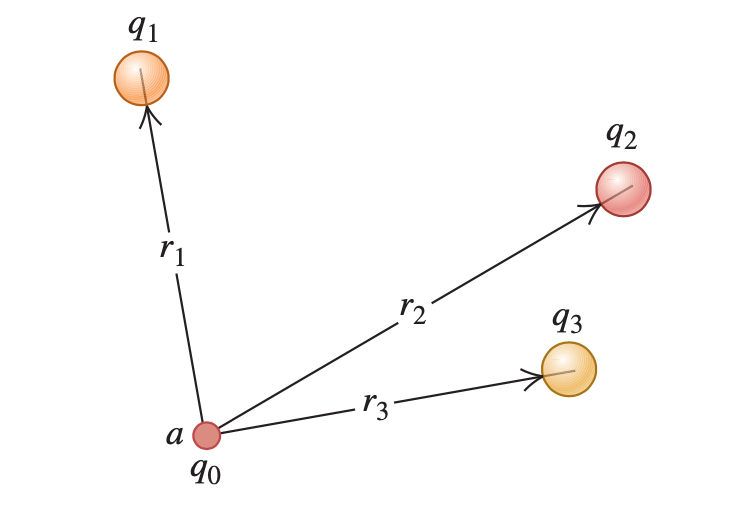
\includegraphics[scale=0.4]{fig/e_potencial_varias}
\label{fig:e_potencial_varias}
\end{figure}

Suponga que el campo eléctrico $\vec{E}$ en el que se desplaza la carga $q_0$ se debe a varias cargas puntuales $q_1, q_2, q_3$, . . . a distancias $r_1, r_2, r_3$, . . . de $q_0$. . El campo eléctrico total en cada punto es la \textit{suma vectorial} de los campos debidos a las cargas individuales, y el trabajo total realizado sobre $q_0$ durante cualquier desplazamiento es la suma de las contribuciones de las cargas individuales. De la ecuación \ref{23.9.e_potencial} se concluye que la energía potencial asociada con la carga de prueba $q_0$ en el punto a en la figura \ref{fig:e_potencial_varias} es la suma \textit{algebraica} (no la suma vectorial).

\begin{equation}\label{23.10}\marginnote{Carga puntual $q_0$ y conjunto de cargas $q_i$}
\boxed{U=\frac{q_0}{4\pi\epsilon_0}\left(\frac{q_1}{r_1}+\frac{q_2}{r_2}+\frac{q_3}{r_3}+\cdots \right)=\frac{q_0}{4\pi\epsilon_0}\sum_{i}\frac{q_i}{r_i}}
\end{equation}

El trabajo efectuado sobre la carga $q_0$ cuando se desplaza de $a$ a $b$ a lo largo de cualquier trayectoria es igual a la diferencia $U_a-U_b$ entre las energías potenciales cuando $q_0$ está en $a$ y 4n $b$.

Se puede representar \textit{cualquier} distribución de carga como un conjunto de cargas puntuales, por lo que la ecuación \ref{23.10} muestra que \textbf{para todo campo eléctrico debido a una distribución de carga estática, la fuerza ejercida por ese campo es conservativa.}

Las ecuaciones \ref{23.9.e_potencial} y \ref{23.10} definen que $U$ es igual a cero cuando todas las distancias $r_1, r_2, . . .$ son infinitas, es decir, cuando la carga de prueba $q_0$ está muy lejos de todas las cargas que producen el campo.

\subsubsection{Interpretación de la energía potencial eléctrica}
Definimos la energía potencial eléctrica en términos del trabajo realizado por el campo eléctrico sobre una partícula con carga que se mueve en el campo. Cuando una partícula se desplaza del punto $a$ al punto $b$, el trabajo que realiza sobre ella el campo eléctrico es $W_{a\to b}=U_a-U_b$. Por lo tanto, la diferencia de energía potencial $U_a-U_b$ es igual al \textit{trabajo que efectúa la fuerza eléctrica cuando la partícula se desplaza de $a$ a $b$}. Cuando $U_a$ es mayor que $U_b$ el campo realiza trabajo positivo sobre la partícula conforme “cae” de un punto de mayor energía potencial ($a$) a otro con menor energía potencial ($b$).



